\section{Introduction}
\label{sec:intro}

% Video LLM is strong and works as a foundation model that can be generalized to different tasks
% What if the task contains additional information, how well these models can do? can we leverage the knowledge in this model for these tasks
% Motivation study shows the foundation model has a strong performance on the benchmarks showing that these knowledge is helpful. -> can we leverage this knowledge in adapting the video models and incooperate the additional information.

Large multimodal models have recently demonstrated remarkable success in video understanding~\cite{li2024llava, Qwen2VL, gpt4}. These models, known as video large language models (Video LLMs), are pre-trained on video and text data, exhibiting significant reasoning capabilities across video understanding tasks. They thus promise to serve as video foundation models, characterized by their potential to adapt to many downstream tasks~\cite{bommasani2021opportunities}. However, many of these tasks involve \textit{side-channel signals in the form of additional modalities or data types} beyond the video-text pairs that Video LLMs are typically trained on. For example, audio-visual question answering (QA)~\cite{alamri2019audiovisualsceneawaredialog} necessitates integrating both video and audio to comprehend content, while 3D QA~\cite{azuma_2022_CVPR} requires reasoning about the 3D scene from a video of a 3D scan. 
\textit{What if a target video task offers side-channel signals different from the pre-training of Video LLMs?}  


\begin{figure}[t!]
    \centering
    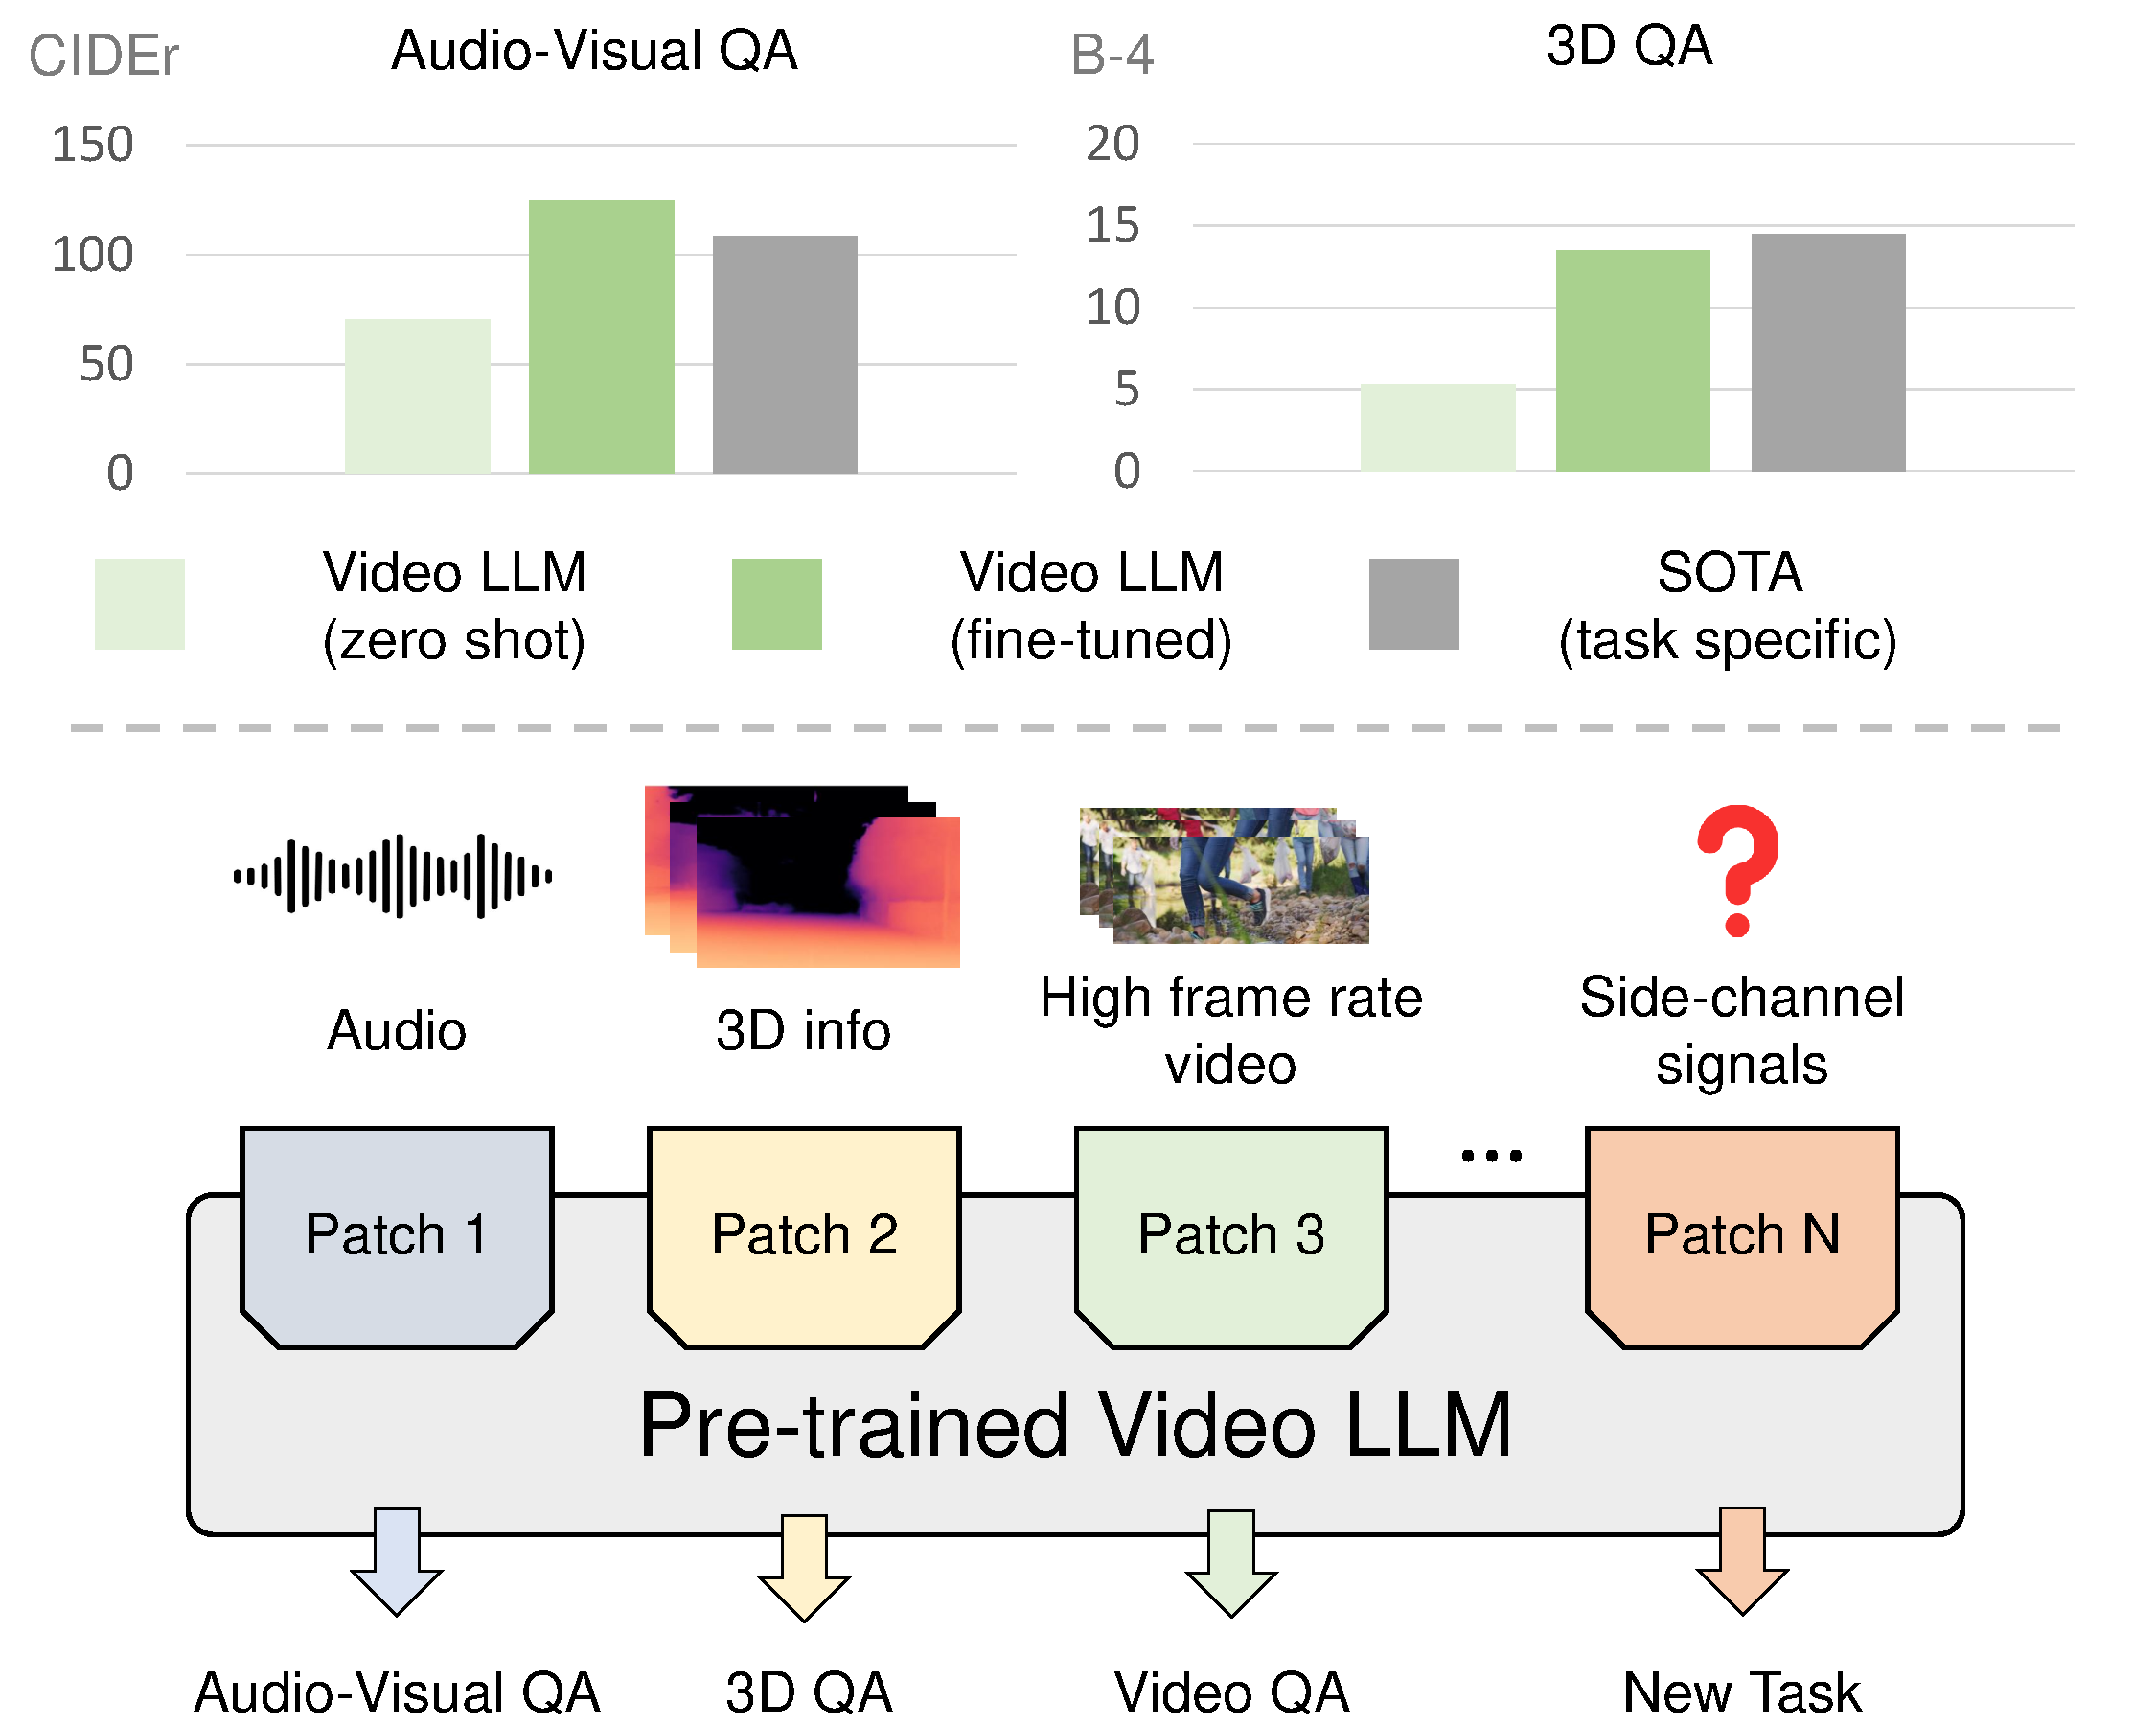
\includegraphics[width=0.95\linewidth]{new_figure_source/pave_teaser.pdf}
    \vspace{-0.5em}
    \caption{\textbf{Top}: Evaluating a Video LLM on audio-visual QA and 3D QA tasks. \textbf{Bottom}: Adapting Video LLMs by adding a small ``patch'' of additional operations and parameters, without changing its existing architecture or vast pre-trained weights.}
    \label{fig:teaser}
    \vspace{-1.5em}
\end{figure}


To answer this question, we begin by evaluating the zero-shot performance of a recent video LLM (LLaVA-OneVision~\cite{li2024llava}) on audio-visual QA~\cite{alamri2019audiovisualsceneawaredialog} and 3D QA tasks~\cite{azuma_2022_CVPR}. Our results, as in Figure~\ref{fig:teaser} (top), show that despite lacking access to audio or 3D-specific data, the Video LLM attains promising performance. Yet, with a similar number of parameters, the Video LLM lags behind those task-specific models that leverage additional side-channel signals. Noting that these task-specific models are indeed trained using the dedicated training sets, for a fair comparison, we further fine-tune the Video LLM on the same training sets yet only with video data (see Figure~\ref{fig:teaser} (top)). Surprisingly, this fine-tuned Video LLM approaches or even surpasses the performance of those specialized models with merely video input. 
Motivated by this observation, our key research question is, \textit{can we leverage the knowledge in pre-trained Video LLMs for such tasks?}

To address this question, we investigate the adaptation of pre-trained Video LLMs to downstream tasks with \textit{side-channel signals}, defined as supplementary signals from additional modalities or data types such as audio, 3D cues, multi-view videos, or high frame rate inputs. 
%supplementary information, such as audio, 3D meshes, multi-view videos, or simply densely sampled video frames, which we termed \textit{side-channel signals}. 
By considering different signals, our formulation addresses key challenges in video understanding. 
For example, considering high frame rate videos as the side-channel explores fundamental questions about video representation~\cite{feichtenhofer2019slowfastnetworksvideorecognition}. Similarly, incorporating multi-view videos, audio, and 3D cues accounts for cross-view and cross-modality reasoning~\cite{grauman2024ego, alamri2019audiovisualsceneawaredialog}.

%Leveraging videos from different perspectives or incorporating audio or 3D data accounts for cross-view and cross-modality reasoning. 

%enables multi-view video recognition~\cite{}, while incorporating audio or 3D data facilitates audio-visual understanding~\cite{alamri2019audiovisualsceneawaredialog} or 3D reasoning~\cite{azuma_2022_CVPR}.

% For example, considering high frame rate videos as side-channel signals delves into the fundamental question about video representation, while using audio or 3D information leads to audio-visual understanding or 3D QA. 

We propose to adapt a pre-trained base Video LLM through \textit{patching} --- adding a lightweight adapter (``patch'') with a small number of additional parameters and operations, and without altering the base model's architecture or vast pre-trained weights (see Figure~\ref{fig:teaser} (bottom)). Inspired by the success of parameter-efficient adapters (\eg, LoRA~\cite{hu2021loralowrankadaptationlarge}) in text and image generation models (\eg, LLMs~\cite{llama3_2, vicuna2023} and diffusion models~\cite{rombach2022highresolutionimagesynthesislatent, polyak2024moviegencastmedia}), this approach allows for flexible customization, and facilitates convenient sharing of the customization by distributing small patches.

To this end, we present \textbf{PAVE}, a framework designed to \underline{P}atch and \underline{A}dapt \underline{V}id\underline{e}o LLMs with side-channel signals. PAVE leverages cross-attention that operates between tokens derived from key video frames (as queries) and tokens from side-channel signals (as keys and values). This operation aligns the visual signal and side-channel signals along the time axis, fuses the signals from both sources, and then updates the input visual tokens to the LLM. In doing so, PAVE integrates side-channel signals with lightweight ``patches,'' while enabling effective adaptation to various downstream tasks without altering pre-trained models. 


%Since the video frames and supplementary signals may have different granularity along the time axis. This operation first leverage the temporal alignment module to align the inputs in time, and split them into multiple mini-batches before applying the cross-attention. During the cross-attention we apply 3-dimension rotary positional embedding (along the time, height, and width axis) for the supplementary signals with spatial dimension, for instance the 3D information and video information.
%Cross-attention aggregates supplementary information into updated visual tokens. These updated visual tokens are then directly summed with the vision tokens in residual connection way, preserving the original model architecture and facilitating efficient inference. In doing so, PAVE allows for the input of supplementary signals, and introduces a small number of parameters and operations with a negligible memory footprint and computing cost, while enabling effective adaptation to various downstream tasks without altering pre-trained models. 

% Yin: shortened to highlight the key findings. Please add refs. 
To evaluate PAVE, We conduct extensive experiments on four video tasks: (1) audio-visual QA, (2) 3D QA, (3) high frame rate video understanding, and (4) multi-view video recognition. Across all tasks, PAVE effectively adapts a base Video LLM~\cite{li2024llava} and consistently outperforms task-specific models. For example, compared to latest task-specific models, PAVE achieves a relative boost of 2\% on the AVQA~\cite{yang2022avqa} dataset for audio-visual QA, 6\% on the SQA3D dataset~\cite{ma2022sqa3d} for 3D QA, 1-5\% across video benchmarks~\cite{fu2024video, li2023mvbench, zhou2025mlvubenchmarkingmultitasklong} when integrating high frame rate videos, and 1\% on the Ego-Exo4D dataset~\cite{grauman2024ego} for multi-view recognition. In all cases, PAVE only adds about 0.1\% of FLOPs and parameters in addition to the base model. Further, we demonstrate that PAVE can support multi-task learning and generalizes well across different Video LLMs.

%and demonstrate that PAVE effectively adapts Video LLMs and outperforms task-specific models across a range of video tasks. For audio-visual QA with audio as side-channel signals, PAVE outperforms the SOTA models~\cite{ye2024catenhancingmultimodallarge, pham2022videodialogconversationobjects} by 44 points, 2\% and 7\% on AVSD, AVQA, and visual split of Music-AVQA, respectively. For 3D QA, where PAVE leverages camera poses and scene depth, PAVE surpasses the state-of-the-art results from the latest 3D MLLM~\cite{zhu2024llava3dsimpleeffectivepathway} by 2-4\%. 
%With the exo-centric videos as side-channel signals, PAVE outperforms the baseline by a clear margin in multi-view video understanding.
%When considering high-framerate videos for video QA, PAVE improves the strong base model~\cite{li2024llava} with 1-5\% boosts on key sub-tasks of widely used benchmarks. In all cases, PAVE only adds less than 1\% of FLOPs and parameters in addition to the base model. Further, we show that PAVE is applicable across multiple Video LLMs. 
%on three different settings: 1. audio-visual understanding with Audio input as supplementary signals. 2. 3D question-answering with additional 3D information. 3. General video understanding with temporal densely sampled video frames as extra input to PAVE. PAVE outperforms the baseline by 28 points on audio-video dataset AVSD, surpassing the previous best model by 3\% on 3DQA benchmark ScanQA, and achieves 1 to 4 \% improvement on different subtasks on VideoMME and MVBench for general video understanding. 

\medskip
Our main \textbf{contributions} are summarized as follows.
\begin{itemize}
    \item We present PAVE, a novel framework to adapt pre-trained Video LLMs for tasks with side-channel signals, greatly extending the capacity of Video LLMs.
    \item We design lightweight ``patches'' that add a small number of parameters and operations to a base model, and keep the original architecture and pre-trained weights unchanged, enabling PAVE's adaptation to varying tasks. 
    %PAVE enables the adaptation by adding a small ``patch'' to a model, leaving the original architecture and pre-trained weights unchanged. 
    %and facilitating the distribution and application of the patches.
    \item We demonstrate that PAVE can be applied across video tasks and Video LLMs, surpassing the performance of strong task-specific models. %to audio-visual and 3D QA tasks with impressive performance, and to enhance video representation within the Video LLM.
\end{itemize}

\begin{comment}
\begin{figure}[t!]
    \centering
    \includegraphics[width=0.8\linewidth]{figures/introduction_2.png}
    \vspace{-1em}
    \caption{Evaluating existing video Large Language Model On ScanQA and AVSD with zero-shot and fine-tuning with LoRA manner. Fine-tuning on the down-steam dataset without using task-specific supplementary data already closes the performance gap or even surpass baselines. This sheds light on better adapting Video LLM to downstream tasks with utilizing supplementary information from downstream tasks. }
    \label{fig:teaser_2}
    \vspace{-1.5em}
\end{figure}
\end{comment}







\begin{comment}
Visual instruction tuning~\cite{liu2023visualinstructiontuning} usher computer vision community into a new era, which use the text as an unified interface to train an vision-language foundation models. Specifically, video-foundation models~\cite{Qwen2VL, li2024llava, zhang2024videoinstructiontuningsynthetic, Maaz2023VideoChatGPT} attract researcher's attention since they are able to understand both static visual sematic and the motion information. 
While human understands the world by using information from multiple sources, these video foundation models usually reasoning by only making use of the static video frames.

To enhance the model capability we aims to tailor them to leverage additional information, which could be come from same modality, video, or from other modality, like audio or motion information. However the existing methods like retraining the model or finetuning the model with LoRA~\cite{hu2021loralowrankadaptationlarge} struggles in handling this setting. while the first one is too expensive for the large language model, the latter one could not take additional information as supplementary.

To fill in the missing piece in this area, we propose 'Patches for Efficient Video Language Model Adaptation with Extra Information' which is adapter with small amount of parameters. PVL contains a simple cross-attention layer which use a vision tokens from the vision encoder of video-Language model as query and additional information as key and value tokens. By applying the explicit temporal Alignment, we aggregate the additional information add it back to the vision token.

\end{comment}
